\chapter{Additional Images}~\label{ch:additionalImages}

% Dreamfusion
\begin{figure}[ht]
    \begin{subfigure}[b]{0.20\textwidth}
        \centering
        \fontsize{9pt}{7pt}\selectfont\text{Iteration 100}\vspace{3cm}
        \fontsize{9pt}{7pt}\selectfont\text{Iteration 5000}\vspace{2.85cm}
        \fontsize{9pt}{7pt}\selectfont\text{Iteration 10000}\vspace{1.95cm}
    \end{subfigure}
    \begin{subfigure}[b]{0.20\textwidth}
        \centering
        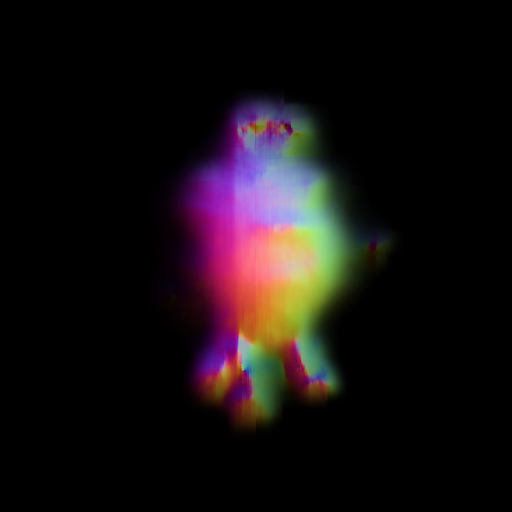
\includegraphics[width=\textwidth]{figures/appendix/dreamfusion_plantrobot_1_part2.png}
        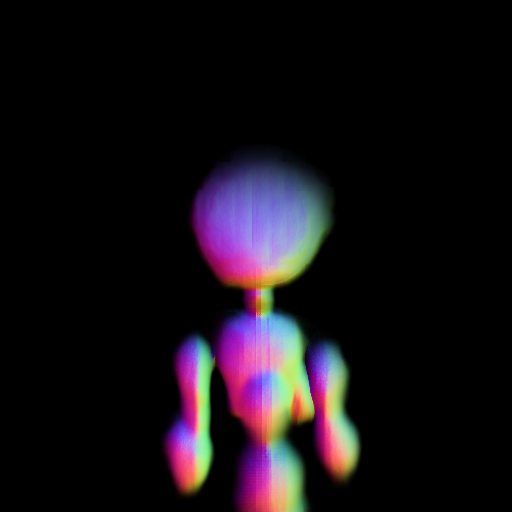
\includegraphics[width=\textwidth]{figures/appendix/dreamfusion_plantrobot_5000_part2.png}
        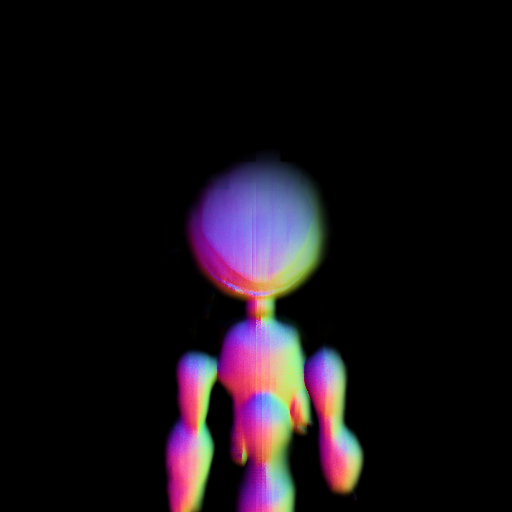
\includegraphics[width=\textwidth]{figures/appendix//dreamfusion_plantrobot_10000_part2.png}
        \caption{}
    \end{subfigure}
    \begin{subfigure}[b]{0.20\textwidth}
        \centering
        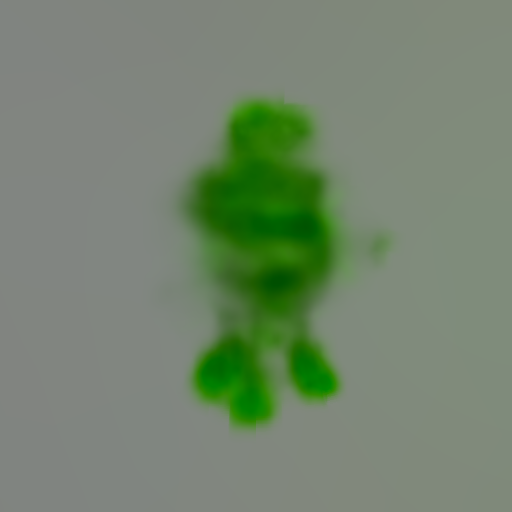
\includegraphics[width=\textwidth]{figures/appendix/dreamfusion_plantrobot_1_part1.png}
        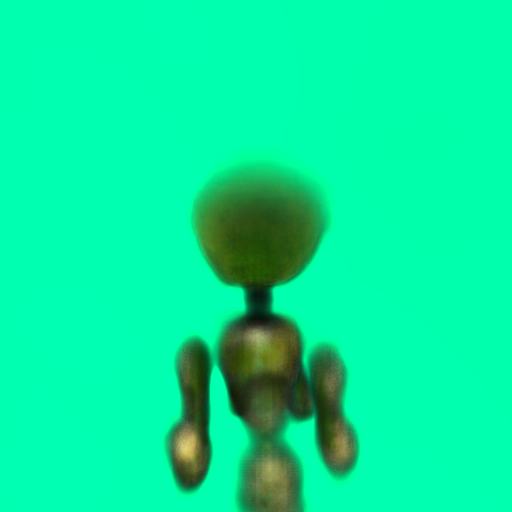
\includegraphics[width=\textwidth]{figures/appendix/dreamfusion_plantrobot_5000_part1.png}
        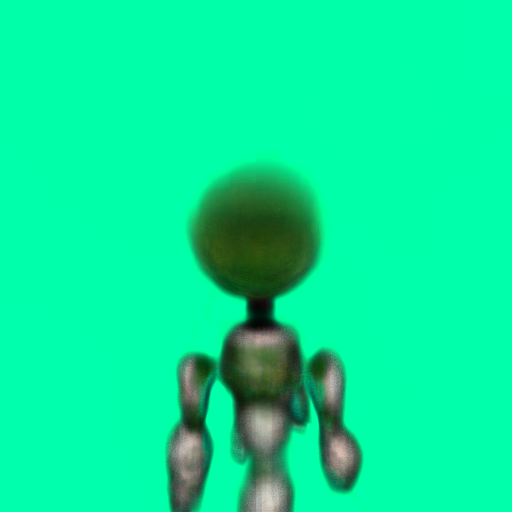
\includegraphics[width=\textwidth]{figures/appendix/dreamfusion_plantrobot_10000_part1.png}
        \caption{}
    \end{subfigure}
    \hspace{.5cm}
    \begin{subfigure}[b]{0.252\textwidth}
        \centering
        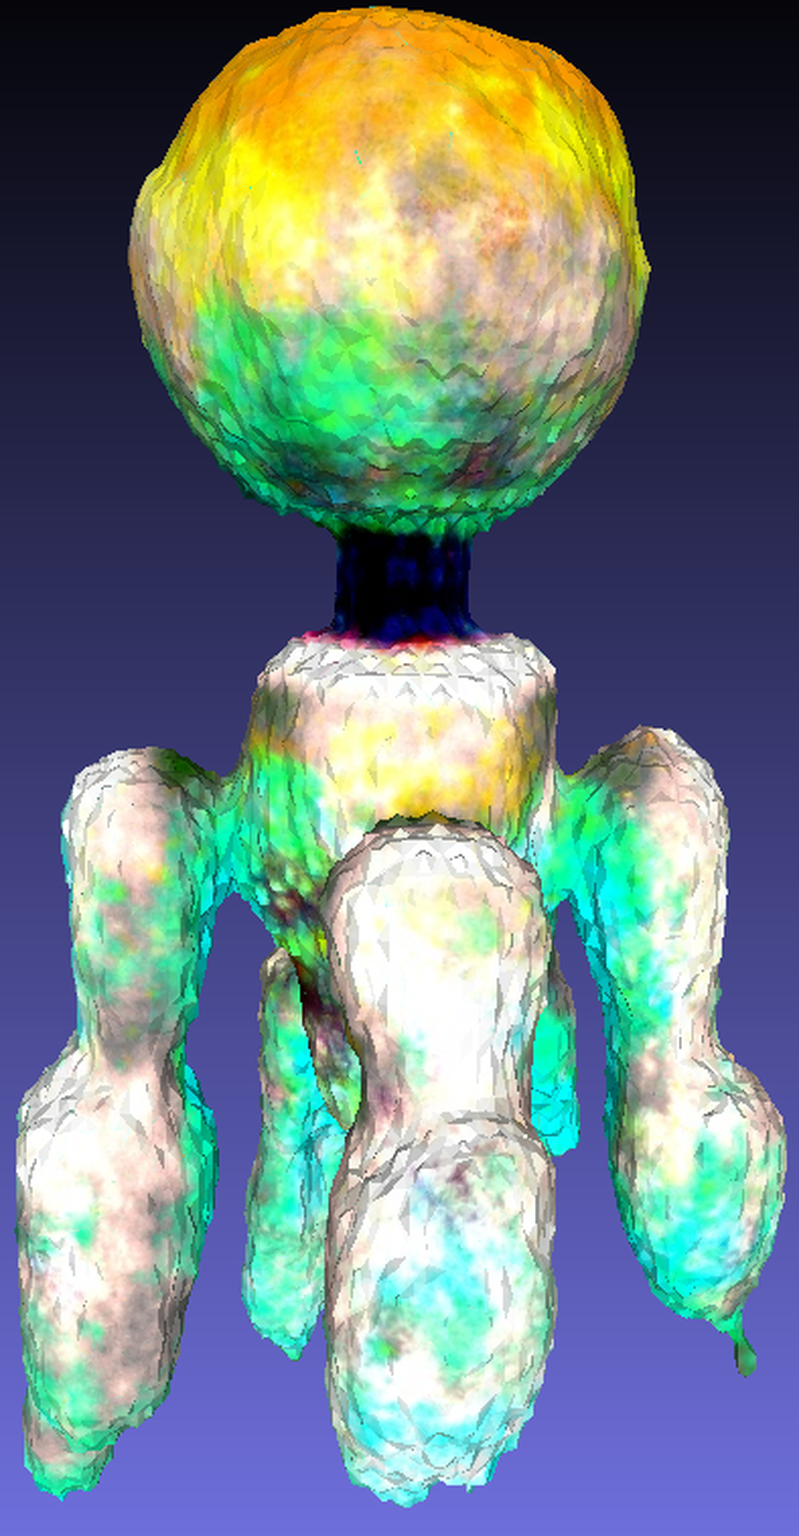
\includegraphics[width=\textwidth]{figures/appendix/dreamfusion_plantrobot_model_resized.png}
        \caption{}
    \end{subfigure}
    \caption{The generation process of DreamFusion using the prompt ``a robot made out of plants'' a second time.}~\label{fig:secondRobotDreamfusion}
\end{figure}



% Fantasia3D
\begin{figure}[ht]
    \centering
    \begin{subfigure}[b]{0.20\textwidth}
        \centering
        \fontsize{9pt}{7pt}\selectfont\text{Iteration 0}\vspace{3cm}
        \fontsize{9pt}{7pt}\selectfont\text{Iteration 5000}\vspace{2.85cm}
        \fontsize{9pt}{7pt}\selectfont\text{Iteration 10000}\vspace{1.95cm}
    \end{subfigure}
    \begin{subfigure}[b]{0.20\textwidth}
        \centering
        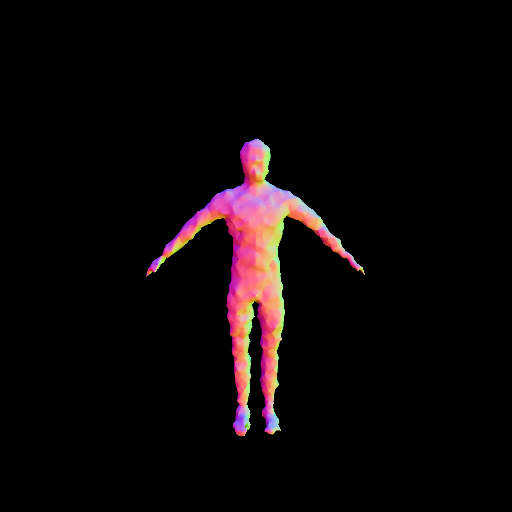
\includegraphics[width=\textwidth]{figures/appendix/fantasia_coarse_robot_0_part2.png}
        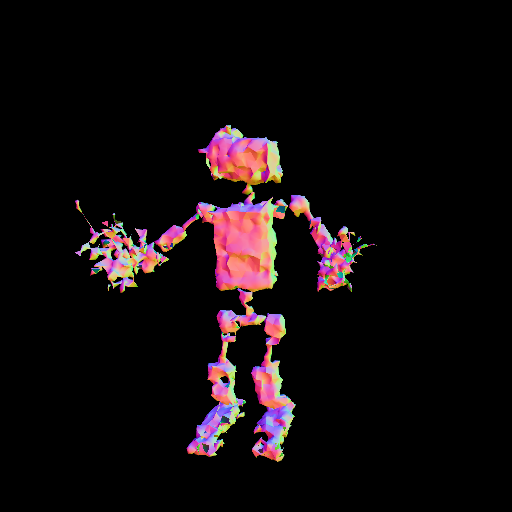
\includegraphics[width=\textwidth]{figures/appendix/fantasia_coarse_robot_5000_part2.png}
        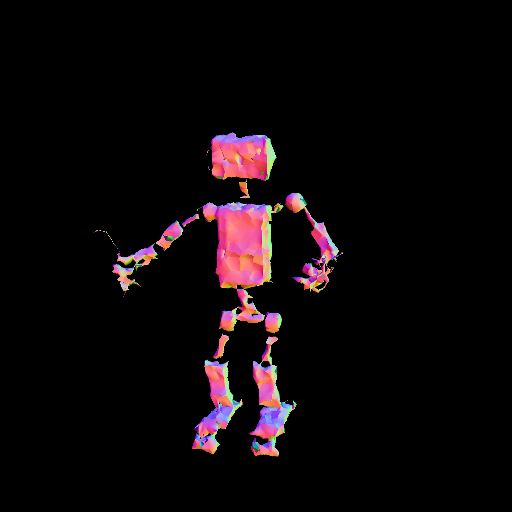
\includegraphics[width=\textwidth]{figures/appendix/fantasia_coarse_robot_10000_part2.png}
        \caption{}
    \end{subfigure}
    \begin{subfigure}[b]{0.20\textwidth}
        \centering
        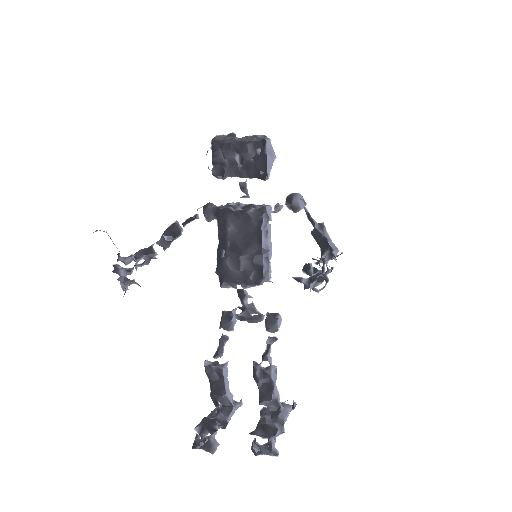
\includegraphics[width=\textwidth]{figures/appendix/fantasia_refine_robot_0_part1.png}
        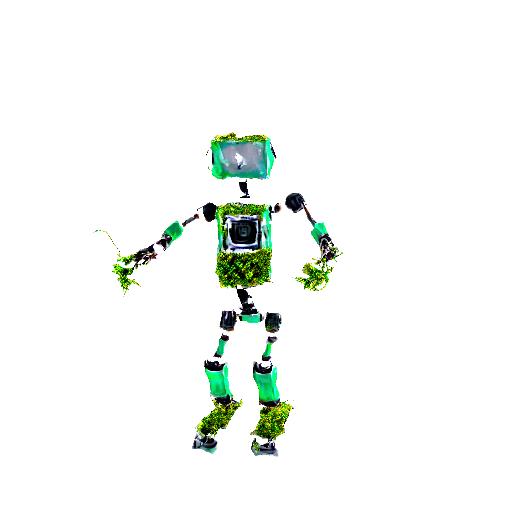
\includegraphics[width=\textwidth]{figures/appendix/fantasia_refine_robot_5000_part1.png}
        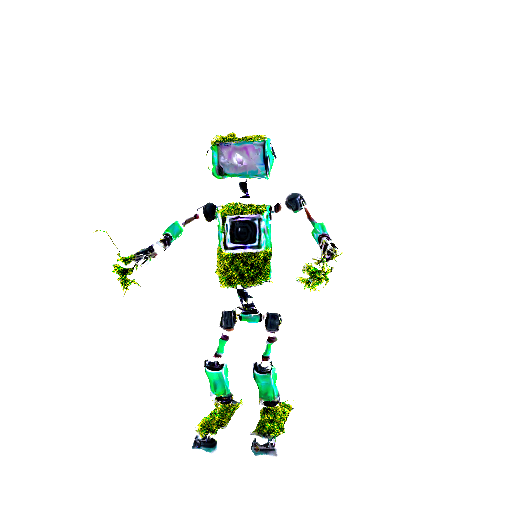
\includegraphics[width=\textwidth]{figures/appendix/fantasia_refine_robot_10000_part1.png}
        \caption{}
    \end{subfigure}
    \begin{subfigure}[b]{0.37\textwidth}
        \centering
        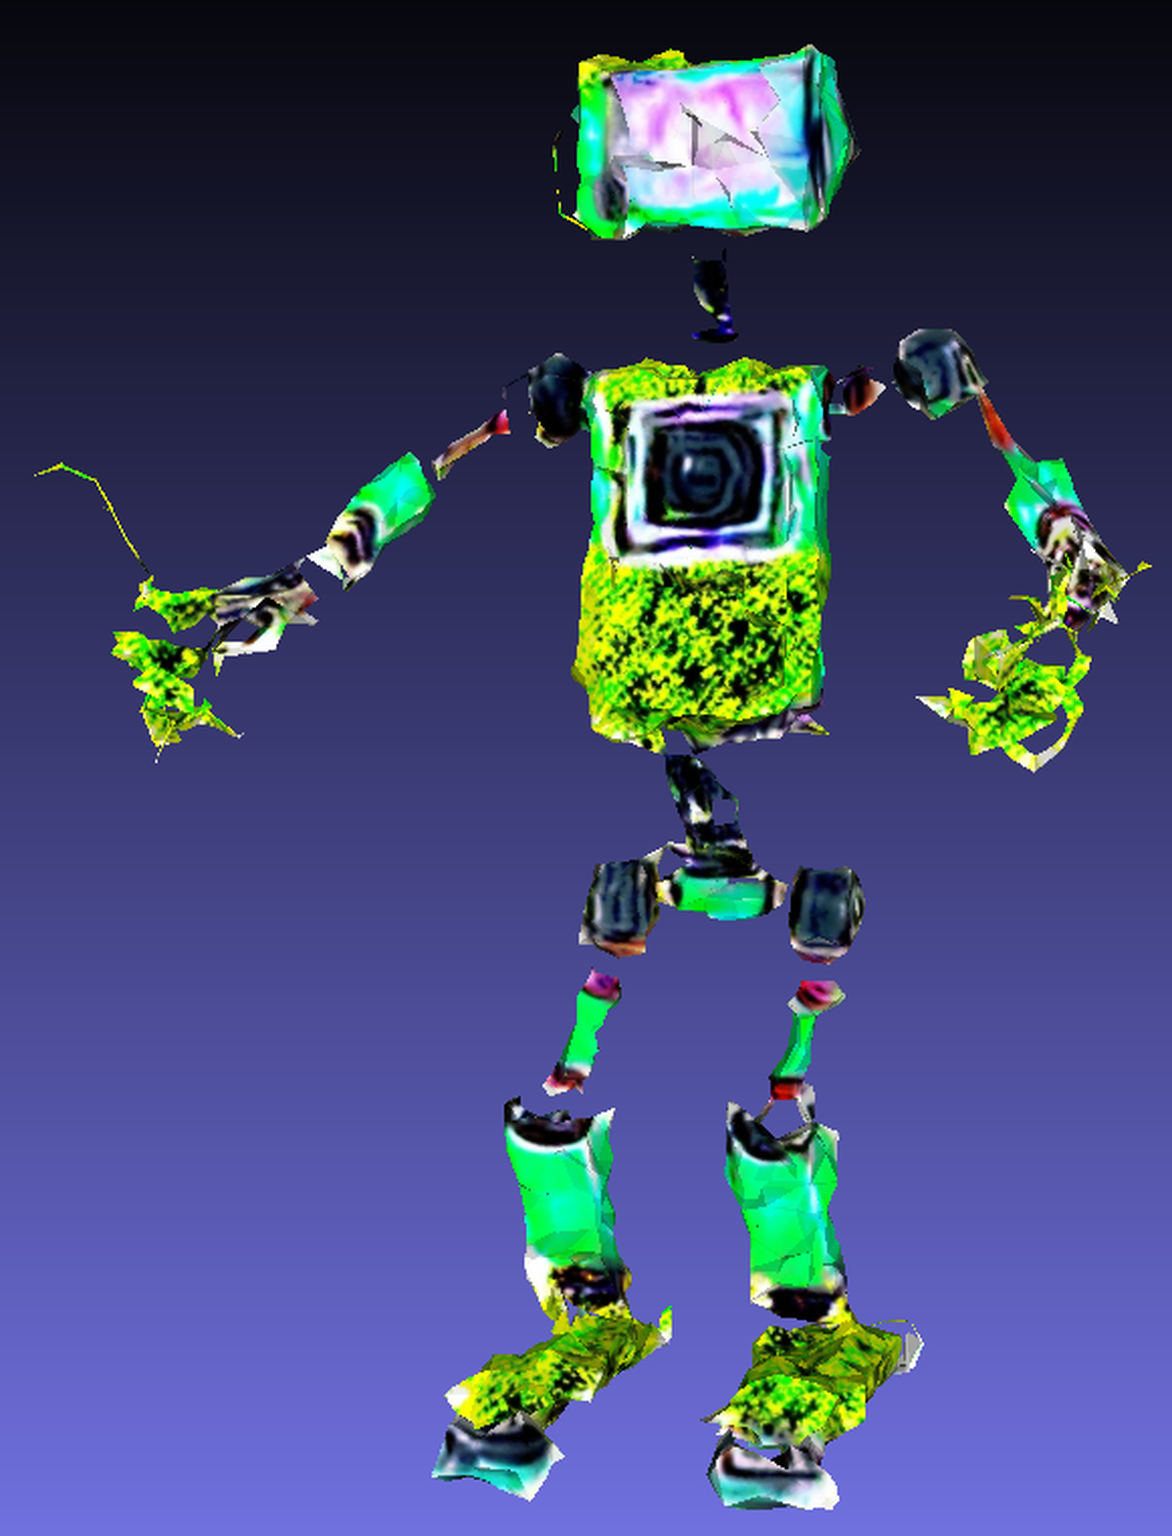
\includegraphics[width=\textwidth]{figures/appendix/fantasia_plantrobot_model_resized.png}
        \caption{}
    \end{subfigure}
    \caption{Initializing Fantasia3D with a coarse mesh representing a basic human figure}~\label{fig:generationFantasia2}
\end{figure}



% Magic123
\begin{figure}[ht]
    \centering
    \begin{subfigure}[b]{0.222\textwidth}
        \centering
        \fontsize{9pt}{7pt}\selectfont\text{Iteration 100}\vspace{.1cm}
        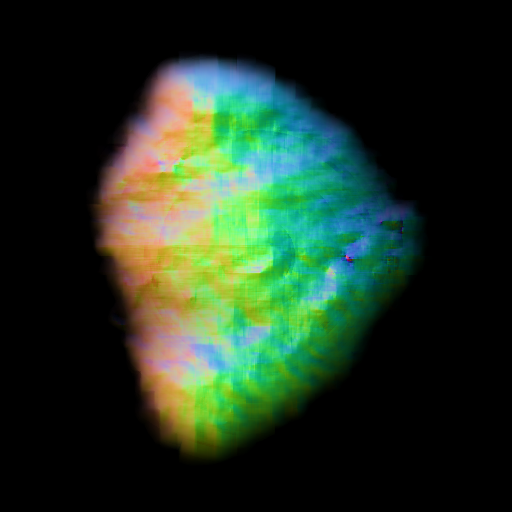
\includegraphics[width=\textwidth]{figures/appendix/magic123_coarse_robot_right_0_part2.png}
        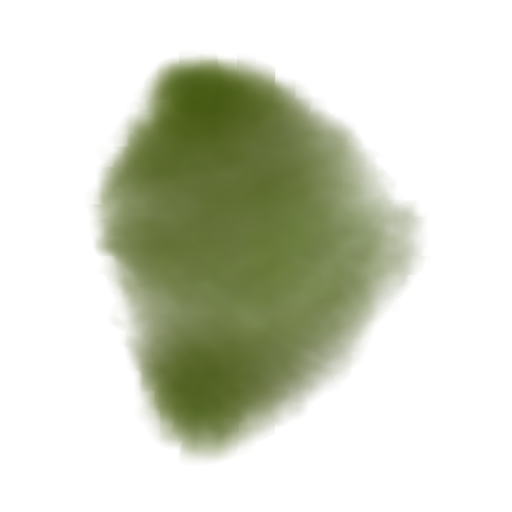
\includegraphics[width=\textwidth]{figures/appendix/magic123_coarse_robot_right_0_part1.png}
        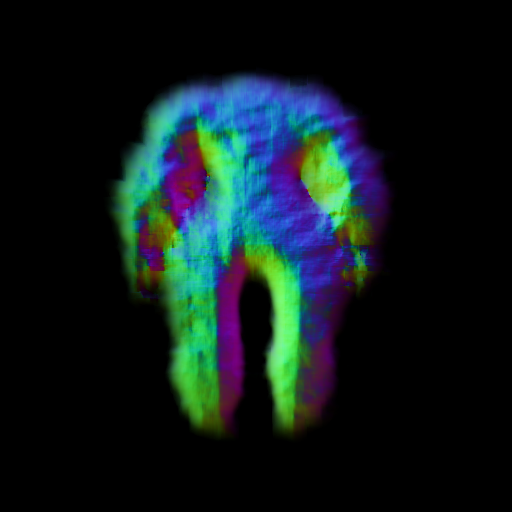
\includegraphics[width=\textwidth]{figures/appendix/magic123_coarse_robot_back_0_part2.png}
        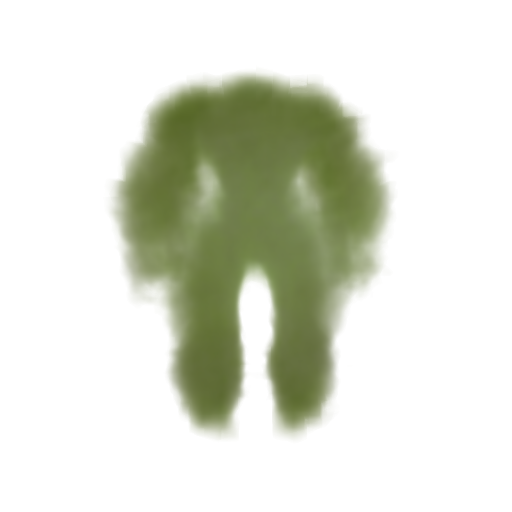
\includegraphics[width=\textwidth]{figures/appendix/magic123_coarse_robot_back_0_part1.png}
        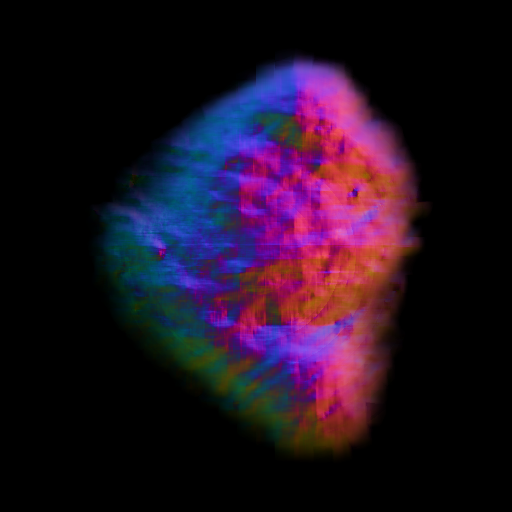
\includegraphics[width=\textwidth]{figures/appendix/magic123_coarse_robot_left_0_part2.png}
        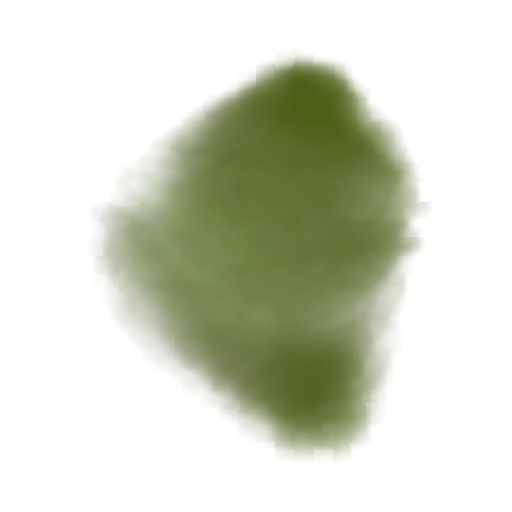
\includegraphics[width=\textwidth]{figures/appendix/magic123_coarse_robot_left_0_part1.png}
        \caption{}
    \end{subfigure}
    \begin{subfigure}[b]{0.222\textwidth}
        \centering
        \fontsize{9pt}{7pt}\selectfont\text{It. 5000}\vspace{.1cm}
        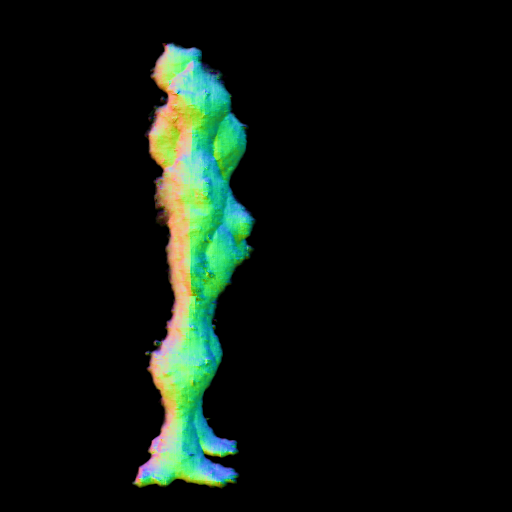
\includegraphics[width=\textwidth]{figures/appendix/magic123_coarse_robot_right_5000_part2.png}
        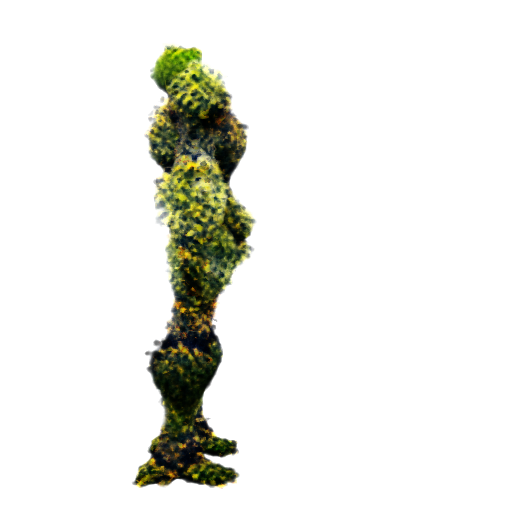
\includegraphics[width=\textwidth]{figures/appendix/magic123_coarse_robot_right_5000_part1.png}
        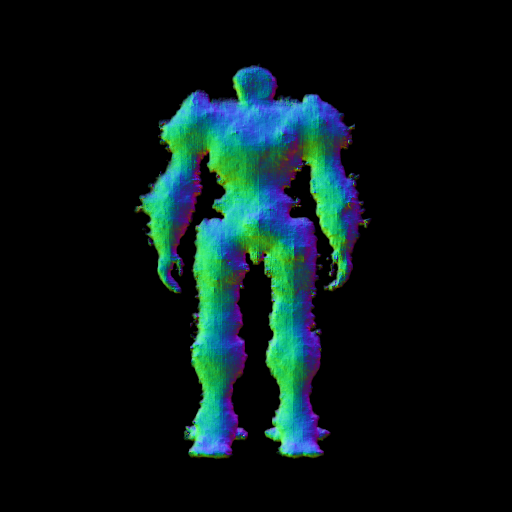
\includegraphics[width=\textwidth]{figures/appendix/magic123_coarse_robot_back_5000_part2.png}
        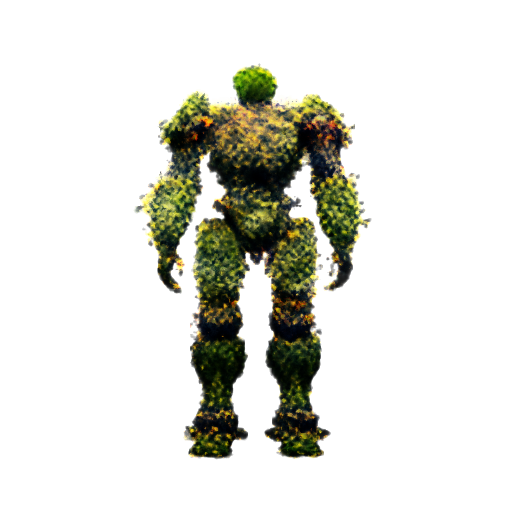
\includegraphics[width=\textwidth]{figures/appendix/magic123_coarse_robot_back_5000_part1.png}
        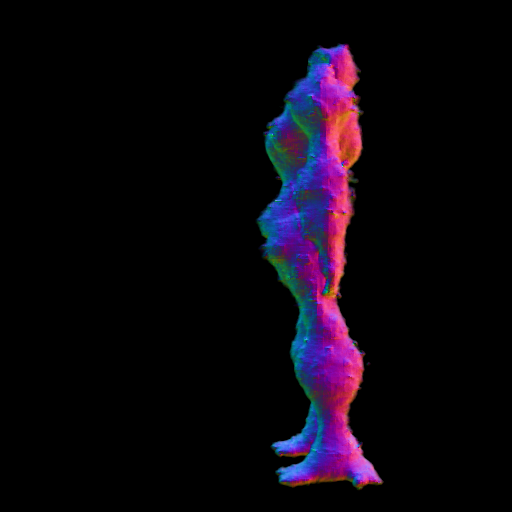
\includegraphics[width=\textwidth]{figures/appendix/magic123_coarse_robot_left_5000_part2.png}
        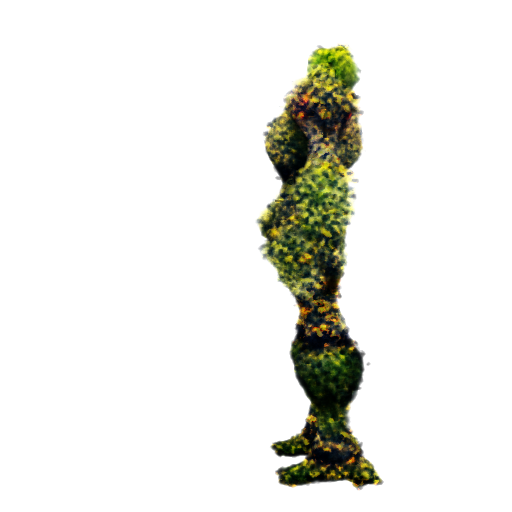
\includegraphics[width=\textwidth]{figures/appendix/magic123_coarse_robot_left_5000_part1.png}
        \caption{}
    \end{subfigure}
    \begin{subfigure}[b]{0.222\textwidth}
        \centering
        \fontsize{9pt}{7pt}\selectfont\text{It. 10000}\vspace{.1cm}
        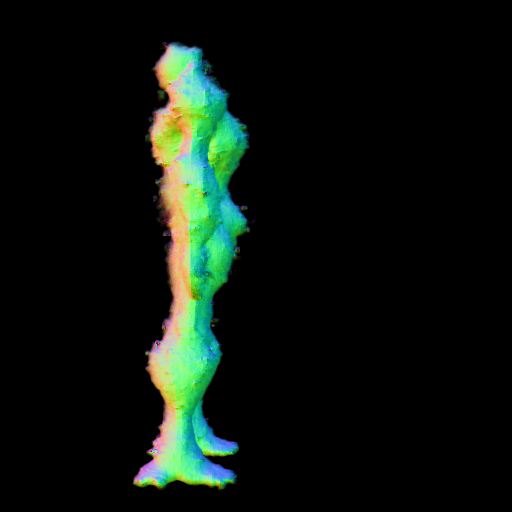
\includegraphics[width=\textwidth]{figures/appendix/magic123_coarse_robot_right_10000_part2.png}
        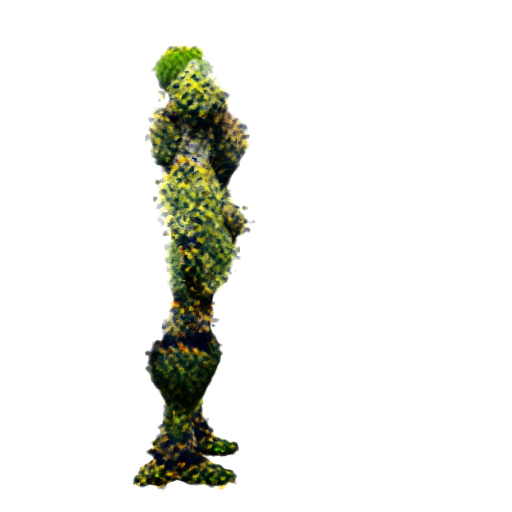
\includegraphics[width=\textwidth]{figures/appendix/magic123_coarse_robot_right_10000_part1.png}
        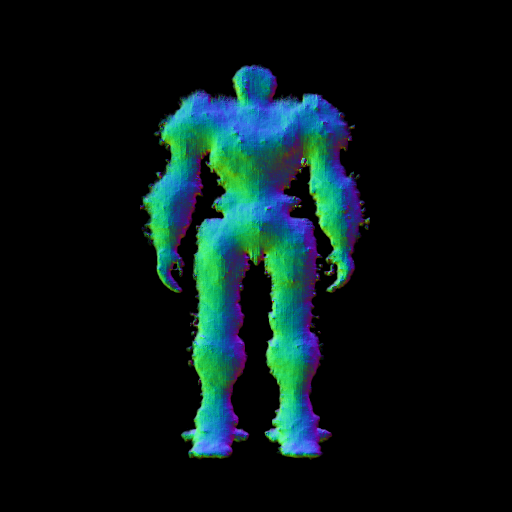
\includegraphics[width=\textwidth]{figures/appendix/magic123_coarse_robot_back_10000_part2.png}
        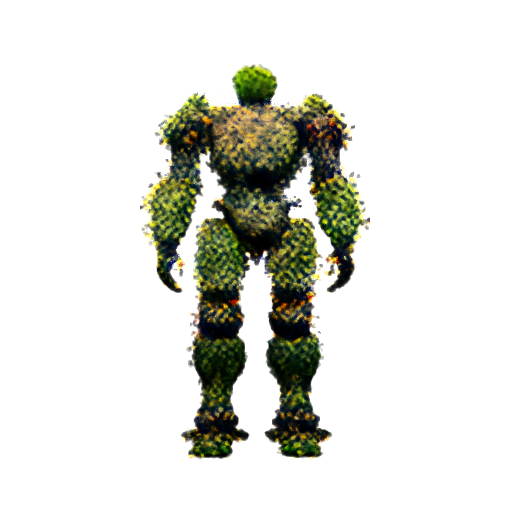
\includegraphics[width=\textwidth]{figures/appendix/magic123_coarse_robot_back_10000_part1.png}
        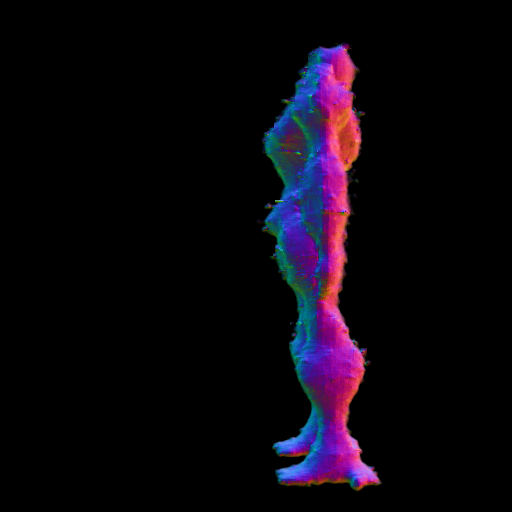
\includegraphics[width=\textwidth]{figures/appendix/magic123_coarse_robot_left_10000_part2.png}
        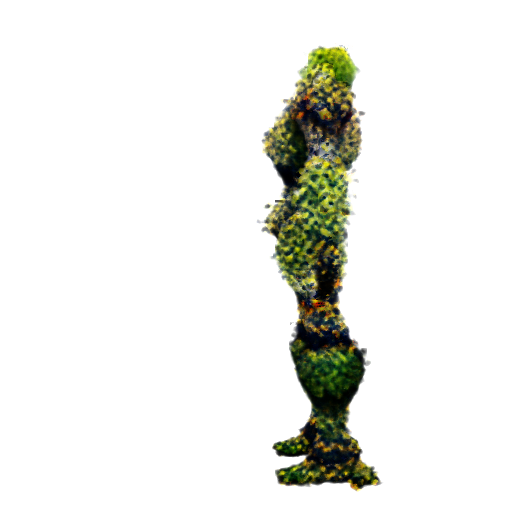
\includegraphics[width=\textwidth]{figures/appendix/magic123_coarse_robot_left_10000_part1.png}
        \caption{}
    \end{subfigure}
    \caption{The coarse in Magic123; From top to bottom: right, back and left view}~\label{fig:generationCoarseMagic123}
\end{figure}

\begin{figure}[ht]
    \centering
    \begin{subfigure}[b]{0.222\textwidth}
        \centering
        \fontsize{9pt}{7pt}\selectfont\text{Iteration 100}\vspace{.1cm}
        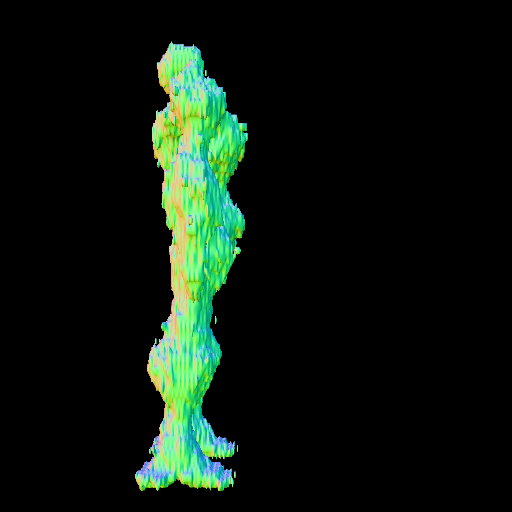
\includegraphics[width=\textwidth]{figures/appendix/magic123_refine_robot_right_0_part2.png}
        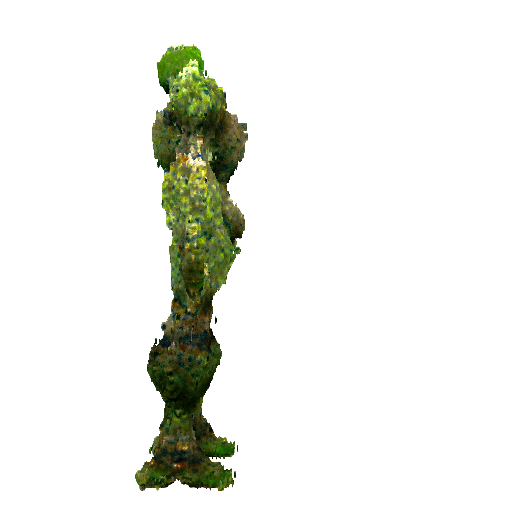
\includegraphics[width=\textwidth]{figures/appendix/magic123_refine_robot_right_0_part1.png}
        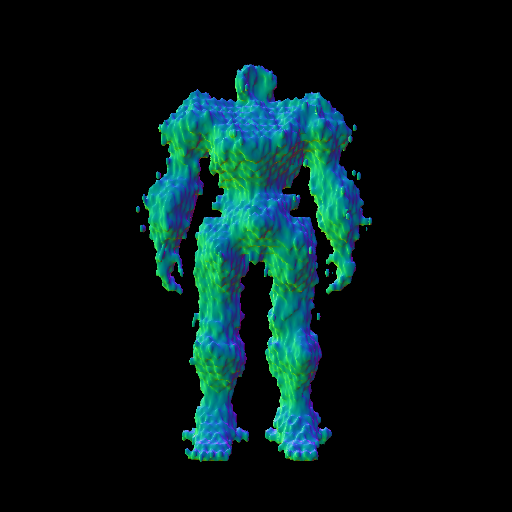
\includegraphics[width=\textwidth]{figures/appendix/magic123_refine_robot_back_0_part2.png}
        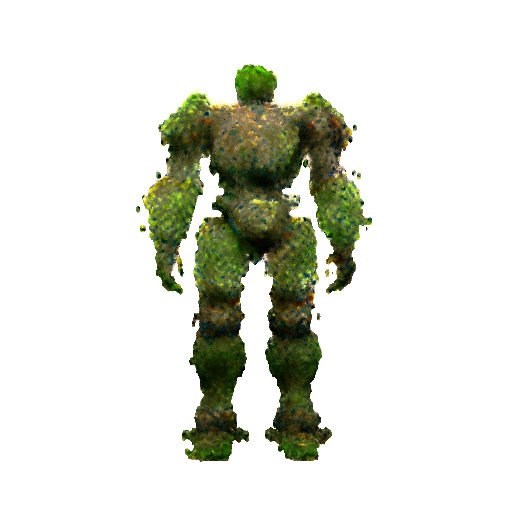
\includegraphics[width=\textwidth]{figures/appendix/magic123_refine_robot_back_0_part1.png}
        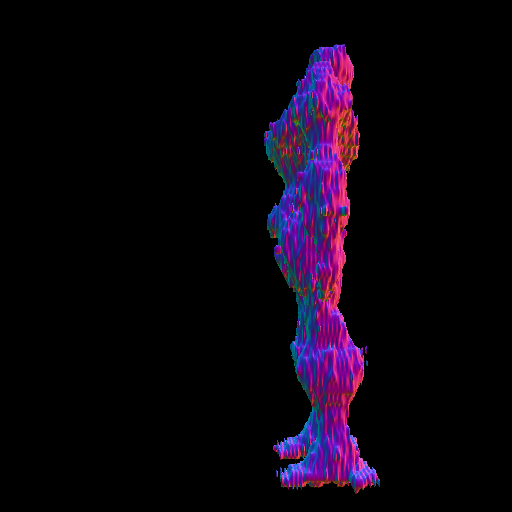
\includegraphics[width=\textwidth]{figures/appendix/magic123_refine_robot_left_0_part2.png}
        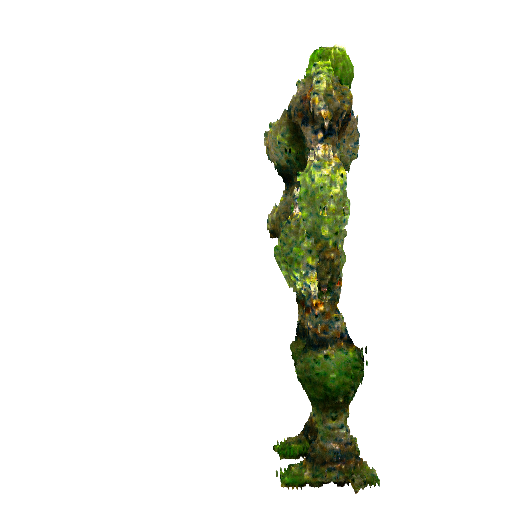
\includegraphics[width=\textwidth]{figures/appendix/magic123_refine_robot_left_0_part1.png}
        \caption{}
    \end{subfigure}
    \begin{subfigure}[b]{0.222\textwidth}
        \centering
        \fontsize{9pt}{7pt}\selectfont\text{It. 5000}\vspace{.1cm}
        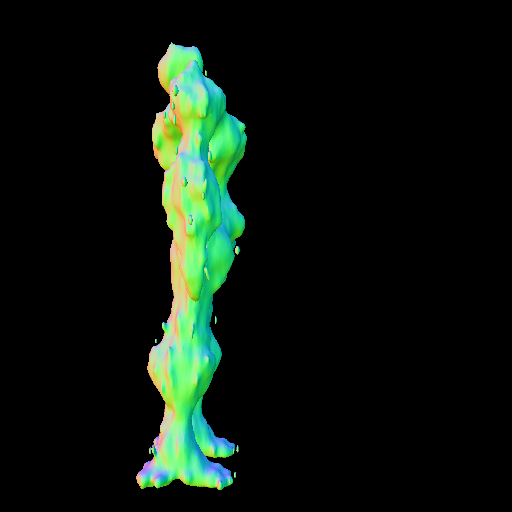
\includegraphics[width=\textwidth]{figures/appendix/magic123_refine_robot_right_5000_part2.png}
        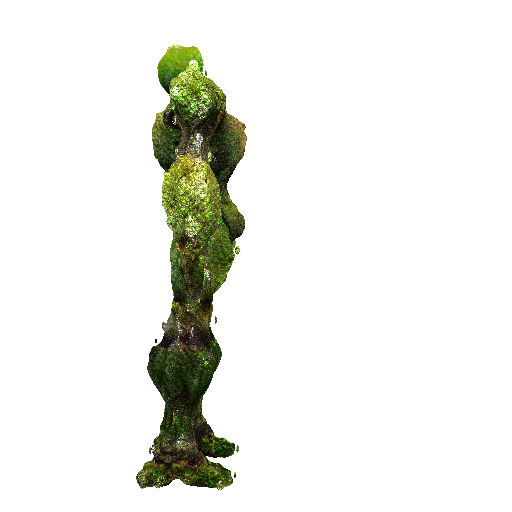
\includegraphics[width=\textwidth]{figures/appendix/magic123_refine_robot_right_5000_part1.png}
        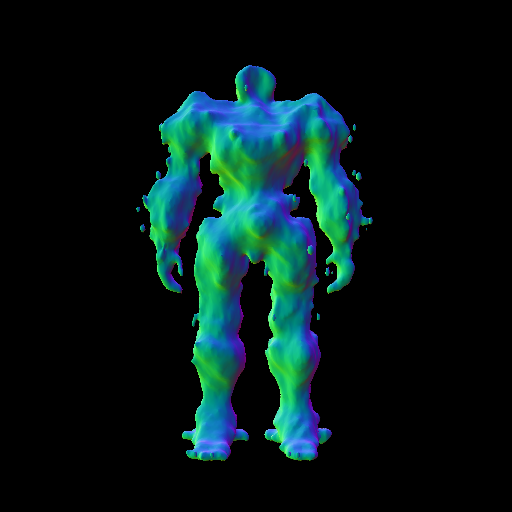
\includegraphics[width=\textwidth]{figures/appendix/magic123_refine_robot_back_5000_part2.png}
        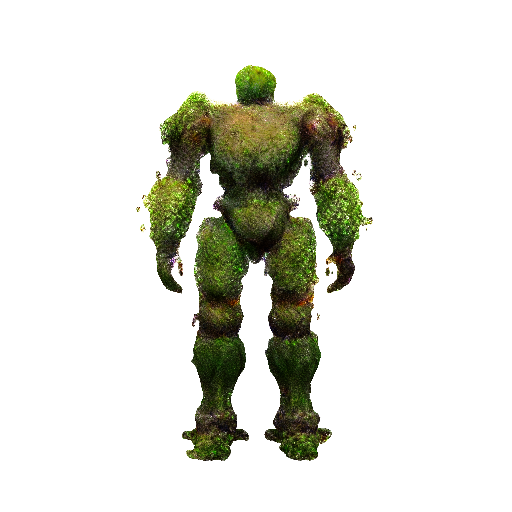
\includegraphics[width=\textwidth]{figures/appendix/magic123_refine_robot_back_5000_part1.png}
        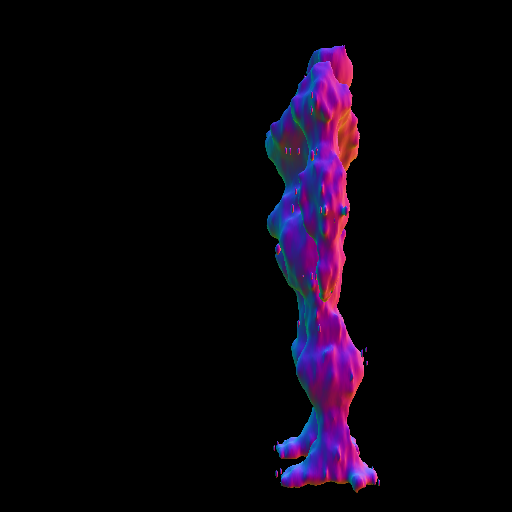
\includegraphics[width=\textwidth]{figures/appendix/magic123_refine_robot_left_5000_part2.png}
        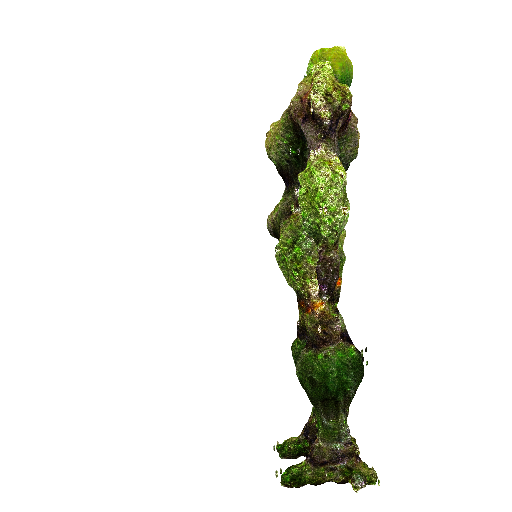
\includegraphics[width=\textwidth]{figures/appendix/magic123_refine_robot_left_5000_part1.png}
        \caption{}
    \end{subfigure}
    \begin{subfigure}[b]{0.222\textwidth}
        \centering
        \fontsize{9pt}{7pt}\selectfont\text{It. 10000}\vspace{.1cm}
        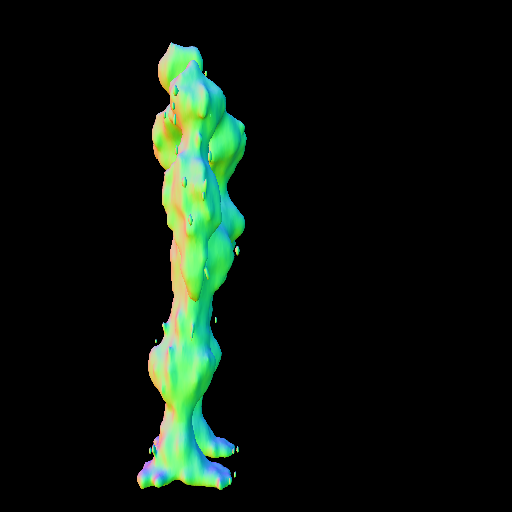
\includegraphics[width=\textwidth]{figures/appendix/magic123_refine_robot_right_10000_part2.png}
        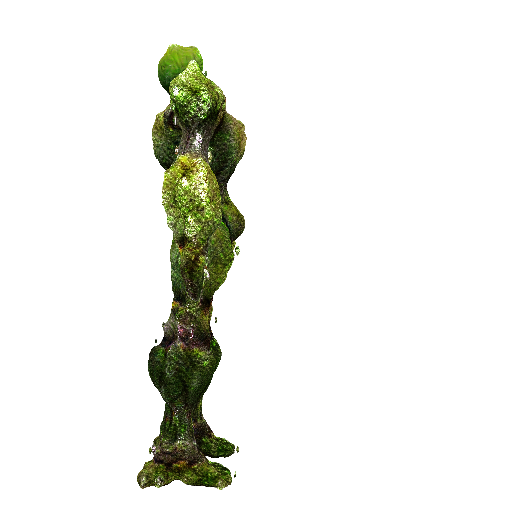
\includegraphics[width=\textwidth]{figures/appendix/magic123_refine_robot_right_10000_part1.png}
        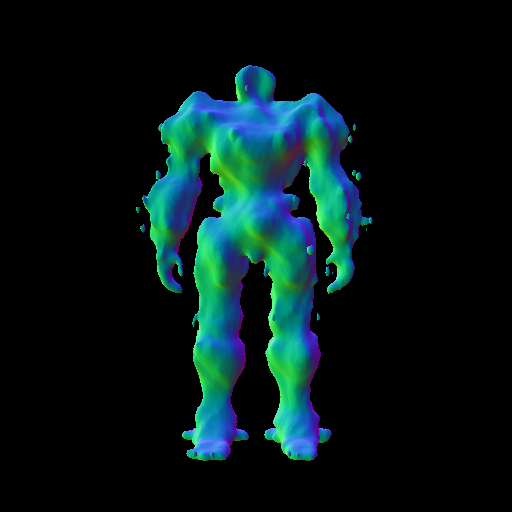
\includegraphics[width=\textwidth]{figures/appendix/magic123_refine_robot_back_10000_part2.png}
        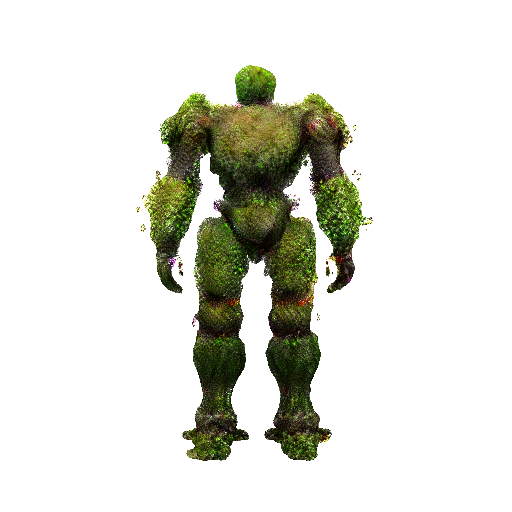
\includegraphics[width=\textwidth]{figures/appendix/magic123_refine_robot_back_10000_part1.png}
        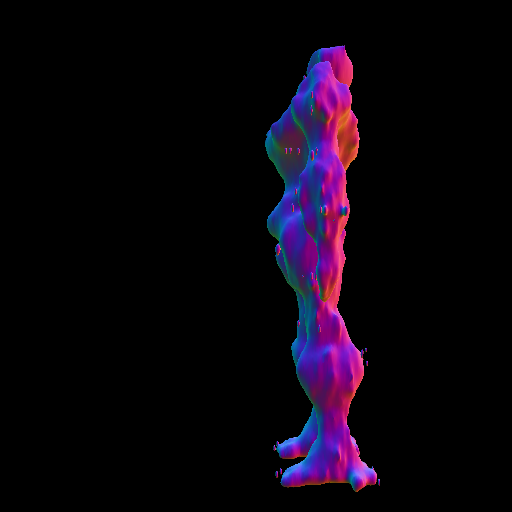
\includegraphics[width=\textwidth]{figures/appendix/magic123_refine_robot_left_10000_part2.png}
        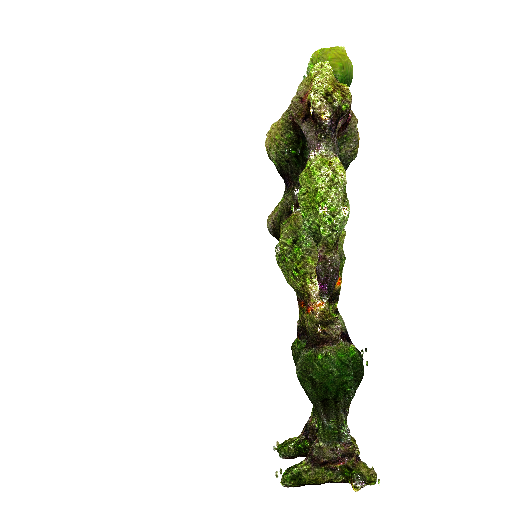
\includegraphics[width=\textwidth]{figures/appendix/magic123_refine_robot_left_10000_part1.png}
        \caption{}
    \end{subfigure}
    \caption{The refine in Magic123; From top to bottom: right, back and left view}~\label{fig:generationRefineMagic123}
\end{figure}



%Wonder3D
\begin{figure}[ht]
    \centering
    \begin{subfigure}[b]{0.3\textwidth}
        \centering
        \includegraphics[width=\textwidth]{figures/appendix/rgb_000_front.png}
        \includegraphics[width=\textwidth]{figures/appendix/normals_000_front.png}
        \caption{}
    \end{subfigure}
    \begin{subfigure}[b]{0.3\textwidth}
        \centering
        \includegraphics[width=\textwidth]{figures/appendix/rgb_000_front_right.png}
        \includegraphics[width=\textwidth]{figures/appendix/normals_000_front_right.png}
        \caption{}
    \end{subfigure}
    \begin{subfigure}[b]{0.3\textwidth}
        \centering
        \includegraphics[width=\textwidth]{figures/appendix/rgb_000_right.png}
        \includegraphics[width=\textwidth]{figures/appendix/normals_000_right.png}
        \caption{}
    \end{subfigure}
    %\hspace{5cm}
    \begin{subfigure}[b]{0.3\textwidth}
        \centering
        \includegraphics[width=\textwidth]{figures/appendix/rgb_000_back.png}
        \includegraphics[width=\textwidth]{figures/appendix/normals_000_back.png}
        \caption{}
    \end{subfigure}
    \begin{subfigure}[b]{0.3\textwidth}
        \centering
        \includegraphics[width=\textwidth]{figures/appendix/rgb_000_left.png}
        \includegraphics[width=\textwidth]{figures/appendix/normals_000_left.png}
        \caption{}
    \end{subfigure}
    \begin{subfigure}[b]{0.3\textwidth}
        \centering
        \includegraphics[width=\textwidth]{figures/appendix/rgb_000_front_left.png}
        \includegraphics[width=\textwidth]{figures/appendix/normals_000_front_left.png}
        \caption{}
    \end{subfigure}
    \caption{Wonder3D initialization of multi-view color images and normals; (a) front, (b) front left, (c) left, (d) back, (e) right, (f) front right}~\label{fig:initializationWonder3D}
\end{figure}






\begin{figure}[ht]
    \centering
    \small
    \begin{subfigure}[b]{0.108\textwidth}
        \centering
        \includegraphics[width=\textwidth]{figures/appendix/bias_rich_dreamfusion.png}
        \caption{}
    \end{subfigure}
    \begin{subfigure}[b]{0.2\textwidth}
        \centering
        \includegraphics[width=\textwidth]{figures/appendix/bias_rich_fantasia3d.png}
        \caption{}
    \end{subfigure}
    \begin{subfigure}[b]{0.12\textwidth}
        \centering
        \includegraphics[width=\textwidth]{figures/appendix/bias_poor_dreamfusion_part1.png}
        \caption{}
    \end{subfigure}
    \begin{subfigure}[b]{0.118\textwidth}
        \centering
        \includegraphics[width=\textwidth]{figures/appendix/bias_poor_magic3d_part1.png}
        \caption{}
    \end{subfigure}
    \begin{subfigure}[b]{0.24\textwidth}
        \centering
        \includegraphics[width=\textwidth]{figures/appendix/bias_poor_fantasia3d_part1.png}
        \caption{}
    \end{subfigure}
    \caption{Parts (a) and (b) illustrate results from DreamFusion and Fantasia3D for the ``rich person'' prompt, while Magic3D failed to converge to a reasonable output. Results for the prompt ``poor person'' by DreamFusion, Magic3D, and Fantasia3D are shown in parts (c-e). DreamFusion's model indicates a clear bias, correlating ``rich person'' with a white figure and ``poor person'' with a person of color. In contrast, Fantasia3D's outputs (b, e) demonstrate no distinct bias towards any socioeconomic status.}~\label{fig:biasRichPoor}
\end{figure}


\begin{figure}[ht]
    \centering
    \small
    \begin{subfigure}[b]{0.23\textwidth}
        \centering
        \includegraphics[width=\textwidth]{figures/appendix/bias_poor_genie_1.png}
        \caption{}
    \end{subfigure}
    \begin{subfigure}[b]{0.1721\textwidth}
        \centering
        \includegraphics[width=\textwidth]{figures/appendix/bias_poor_genie_2.png}
        \caption{}
    \end{subfigure}
    \begin{subfigure}[b]{0.172\textwidth}
        \centering
        \includegraphics[width=\textwidth]{figures/appendix/bias_poor_genie_3.png}
        \caption{}
    \end{subfigure}
    \begin{subfigure}[b]{0.175\textwidth}
        \centering
        \includegraphics[width=\textwidth]{figures/appendix/bias_poor_genie_4.png}
        \caption{}
    \end{subfigure}

    \begin{subfigure}[b]{0.218\textwidth}
        \centering
        \includegraphics[width=\textwidth]{figures/appendix/bias_rich_genie_1.png}
        \caption{}
    \end{subfigure}
    \begin{subfigure}[b]{0.15\textwidth}
        \centering
        \includegraphics[width=\textwidth]{figures/appendix/bias_rich_genie_2.png}
        \caption{}
    \end{subfigure}
    \begin{subfigure}[b]{0.16\textwidth}
        \centering
        \includegraphics[width=\textwidth]{figures/appendix/bias_rich_genie_3.png}
        \caption{}
    \end{subfigure}
    \begin{subfigure}[b]{0.097\textwidth}
        \centering
        \includegraphics[width=\textwidth]{figures/appendix/bias_rich_genie_4.png}
        \caption{}
    \end{subfigure}
    \caption{When LumaAI's Genie is prompted with ``poor person'', the results (a-d) predominantly depict male figures of color, while the ``rich person'' prompt (e-h) yields exclusively white male figures. This disparity indicates racial and gender biases within the generative models.}~\label{fig:biasGenieRichPoor}
\end{figure}




% Original Images

\begin{figure}[ht]
    \centering
    \small
    \begin{subfigure}[b]{0.3\textwidth}
        \centering
        \includegraphics[width=\textwidth]{figures/appendix/dreamfusion_a_yorkie_dog_wearing_extremely_cool_sneakers.PNG}
        \caption{}
    \end{subfigure}
    \begin{subfigure}[b]{0.3\textwidth}
        \centering
        \includegraphics[width=\textwidth]{figures/appendix/dreamfusion_an_astronaut_playing_the_violin.PNG}
        \caption{}
    \end{subfigure}
    \begin{subfigure}[b]{0.3\textwidth}
        \centering
        \includegraphics[width=\textwidth]{figures/appendix/dreamfusion_neuschwanstein.PNG}
        \caption{}
    \end{subfigure}
    \caption{Possible results from DreamFusion using the original settings. Images taken from~\citep{pooleDreamfusion}. Part (a) prompt: ``a yorkie dog wearing extremely cool sneakers'', part (b) prmopt: ``an astronaut playing the violin'' and the prompt for part (c): ``Neuschwanstein Castle, areal view''.}\label{fig:dreamfusionOriginal}
\end{figure}


\begin{figure}[ht]
    \centering
    \small
    \begin{subfigure}[b]{0.187\textwidth}
        \centering
        \includegraphics[width=\textwidth]{figures/appendix/magic3D_astronaut.PNG}
        \caption{}
    \end{subfigure}
    \begin{subfigure}[b]{0.5\textwidth}
        \centering
        \includegraphics[width=\textwidth]{figures/appendix/magic3D_schloss_neuschwanstein.PNG}
        \caption{}
    \end{subfigure}
    \caption{Results derived from Magic3D \citep{lin2023magic3d} using the original settings.}\label{fig:magic3DOriginal}
\end{figure}


\begin{figure}[ht]
    \centering
    \small
    \begin{subfigure}[b]{0.3\textwidth}
        \centering
        \includegraphics[width=\textwidth]{figures/appendix/fantasia_a_mug_of_hot_chocolate_with_whipped_cream_and_marshmallows.PNG}
        \caption{}
    \end{subfigure}
    \begin{subfigure}[b]{0.3\textwidth}
        \centering
        \includegraphics[width=\textwidth]{figures/appendix/fantasia_a_vintage_record_player.PNG}
        \caption{}
    \end{subfigure}
    \begin{subfigure}[b]{0.3\textwidth}
        \centering
        \includegraphics[width=\textwidth]{figures/appendix/fantasia_ahighly_detailed_sandcastle.PNG}
        \caption{}
    \end{subfigure}
    \caption{Fantasia3D's realistic 3D renderings: Images from \citep{chen2023fantasia3d}. Part (a) using the prompt ``a mug of hot chocolate with whipped cream and marshmallows'', part (b) ``a vintage record player'', and part (c) ``a highly detailed sandcastle''.}\label{fig:fantasia3DOriginal}
\end{figure}

\begin{figure}[ht]
    \centering
    \small
    \begin{subfigure}[b]{0.9\textwidth}
        \centering
        \includegraphics[width=\textwidth]{figures/appendix/magic123_examples.PNG}
        \caption{}
    \end{subfigure}
    \caption{Diverse 3D models from Magic123, demonstrating varied rendering capabilities. Figure taken from \citep{qian2023magic123}. The first image of a series is the input image, the middle image is the 3D color perspective and the right part are the density maps.}\label{fig:magic123Original}
\end{figure}


\begin{figure}[ht]
    \centering
    \small
    \begin{subfigure}[b]{0.9\textwidth}
        \centering
        \includegraphics[width=\textwidth]{figures/appendix/wonder3d_animal_examples.PNG}
        \caption{}
    \end{subfigure}
    \caption{Wonder3D's high-quality animal results from the official paper \citep{long2023wonder3d}.}\label{fig:wonder3dOriginal}
\end{figure}


\chapter{Adaptive Modifications in Threestudio Implementations}\label{ch:differences}



In the Threestudio project's adaptation of DreamFusion, Magic3D, Fantasia3D, and Magic123, several structural changes were implemented, distinguishing them from their official paper counterparts. These differences stated here are directly taken as given in the Threestudio GitHub Project Page~\citep{threestudio2023}: 

For DreamFusion, open-source Text-to-Image models like StableDiffusion and DeepFloyd IF are used instead of Imagen as in the original paper. A lower guidance scale of 20 is applied for DeepFloyd IF, as opposed to 100 used for Imagen. The normalization of albedo color deviates from the sigmoid approach; it's simply scaled from a range of [-1,1] to [0,1] to aid in convergence. The project employs HashGrid encoding and uniform ray sampling, contrasting with Integrated Positional Encoding and MipNeRF360's sampling strategy in the paper. Camera settings and density initialization are adopted from Magic3D, which slightly differ from the DreamFusion paper. Additionally, there are variations in hyperparameters like the weighting of loss terms.

In Magic3D's implementation within Threestudio, open-source T2I models are used for the coarse stage, as opposed to eDiff-I in the paper. The guidance scale for DeepFloyd IF is set at 20, contrasting with the paper's 100 for eDiff-I. The coarse stage utilizes analytic normal instead of predicted normal and includes orientation loss as in DreamFusion, which the paper does not incorporate. There are also omissions and potential differences in aspects like the weighting of loss terms and DMTet grid resolution.

For Fantasia3D, tangent-space normal perturbation is enabled by default, diverging from the paper's approach, but can be disabled with specific system settings. Magic123 in Threestudio is an unofficial re-implementation, sharing the overall idea with the official version but differing in aspects such as hyperparameters. It doesn't support Textual Inversion, necessitating a text prompt for training. These modifications reflect Threestudio's approach to adapting and optimizing these models within their resource constraints and technological framework.

Additionally, specific technical parameters were set to streamline the generation flow of various models, occasionally diverging from the original methods to minimize computational costs and ensure operational feasibility. An example of this adaptation is seen in the Fantasia3D project \citep{chen2023fantasia3d}, where the original configuration used \(512\times512\) images for the geometry stage and scaled up to \(2048\times2048\) for the appearance stage, a setup requiring substantial processing power. Modifying these parameters could potentially lead to improved outcomes, but at the expense of significantly increased computational demands, a constraint particularly relevant when working with platforms like Colab. Therefore, these values were maintained as originally set. It is important to point out that the adjustments mentioned here, such as the image resolution and optimizer settings, represent only a fraction of the extensive hyperparameter changes implemented in the Threestudio versions of these models, reflecting a comprehensive optimization approach tailored to specific resource constraints.

Each model was assigned a seed value of 0 to ensure consistent reproducibility. DreamFusion operates on a \(64\times64\) resolution, whereas Magic3D uses \(64\times64\) in its coarse stage and \(512\times512\) in the refine stage. Fantasia3D is set to \(512\times512\) in both its geometry and appearance stages. Magic123 employs \(128\times128\) images for its coarse stage and upgrades to \(512\times512\) for the refine stage. Wonder3D, on the other hand, uses \(256\times256\) for its coarse stage and escalates to \(1024\times1024\) in the refine stage, indicating the highest resolution among these models. The optimizer learning rate is uniformly set at 0.01 across all models. DreamFusion, Magic3D, and Magic123 utilize the Adam optimizer, whereas Fantasia3D and Wonder3D employ the AdamW optimizer. The latter is preferred for its enhanced handling of weight decay and ability to improve model generalization. Regarding precision, all models, except Wonder3D, adopt a 16-mixed precision approach, which integrates 16-bit computational efficiency with 32-bit accuracy. Wonder3D, on the other hand, opts for 16-bit precision, prioritizing faster computation at the possible expense of precision.